\documentclass[a4paper]{scrartcl}

\usepackage[
    fancytheorems, 
    fancyproofs, 
    noindent, 
]{adam}

\usepackage{physics}
\usepackage{amsmath}
\usepackage{tikz}
\usepackage{mathdots}
\usepackage{yhmath}
\usepackage{cancel}
\usepackage{color}
\usepackage{siunitx}
\usepackage{array}
\usepackage{multirow}
\usepackage{amssymb}
\usepackage{gensymb}
\usepackage{tabularx}
\usepackage{extarrows}
\usepackage{booktabs}
\usetikzlibrary{fadings}
\usetikzlibrary{patterns}
\usetikzlibrary{shadows.blur}
\usetikzlibrary{shapes}


\title{Analysis and Topology}
\author{Adam Kelly (\texttt{ak2316@cam.ac.uk})}
\date{\today}

\allowdisplaybreaks

\begin{document}

\maketitle

This course is a second course in Analysis and a first course in Topology. 
We will study both concrete results over $\R$ and $\C$ concerning uniform convergence and continuity, and we will also move to more abstract settings to discuss metric and topological spaces, completeness, connectedness and compactness.

This article constitutes my notes for the `Analysis and Topology' course, held in Michaelmas 2021 at Cambridge. These notes are \emph{not a transcription of the lectures}, and differ significantly in quite a few areas. Still, all lectured material should be covered.



\tableofcontents

% \section{Introduction}

% \subsection{Outline of the Course}

% This is a second course in Analysis and a first course in Topology. 

% \begin{enumerate}
%     \item Uniform convergence and uniform continuity
%     \item Metric spaces
%     \item Completeness and the contraction mapping theorem
%     \item Topological spaces
%     \item Connectedness
%     \item Compactness
%     \item Differentiation and the inverse function theorem
% \end{enumerate}

% \subsection{Prerequisites}

% Of course the Analysis I course from Part IA is going to assumed knowledge.

% \subsection{Books}

% Burkill \& Burkill and Sutherland are both good. Sutherland has a good motivation about abstraction.

% \subsection{Example Sheets}

% Plus questions are not exam questions.

\section{Uniform Convergence and Uniform Continuity} 

\subsection{Uniform Convergence}
Recall the notion of convergence for a sequence in $\R$ or $\C$:

\begin{definition}[Convergence of a Sequence]
    A sequence $a_{1}, a_{2}, \cdots \in \mathbb{R}$ is said to \vocab{converge} to the limit $a$ if given any $\epsilon>0$, we can find an integer $N$ such that $\left|a_{n}-a\right|<\epsilon$ for all $n \geq N$. We write $a_{n} \rightarrow a$ as $n \rightarrow \infty$
\end{definition}

That is, given any $\varepsilon$, there is some point in the sequence after which the terms of the sequence are $\varepsilon$ close to $a$. 

Our aim is going to define a similar notion to make sense of $f_n \rightarrow f$, where $f_n$ is a sequence of functions.

\begin{definition}[Uniform Convergence]
    A sequence of functions $f_1, f_2, \dots$ with $f_i : S \rightarrow \R$ is said to \vocab{converge uniformly} on $S$ to a function $f:S \rightarrow \R$ if given any $\varepsilon > 0$, we can find an integer $N$ such that $|f_n(x) - f(x)| < \varepsilon$, for any $x \in S$.
\end{definition}

\begin{remark}
    In the above definition, our $N$ can depend only on $\varepsilon$, and must be independent of the particular choice of $x \in S$. This is why we call this \emph{uniform} convergence -- because the property has to hold uniformly across the domain. 
\end{remark}

\begin{center}
    


    \tikzset{every picture/.style={line width=0.75pt}} %set default line width to 0.75pt        

    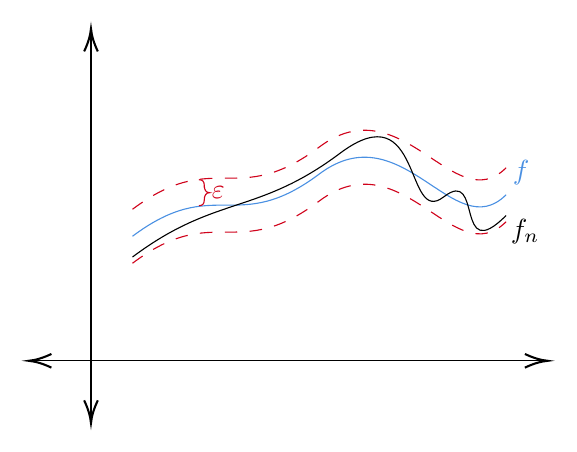
\begin{tikzpicture}[x=0.75pt,y=0.75pt,yscale=-1,xscale=1]
    %uncomment if require: \path (0,300); %set diagram left start at 0, and has height of 300
    
    %Straight Lines [id:da15070589522945865] 
    \draw    (120,42) -- (120,228) ;
    \draw [shift={(120,230)}, rotate = 270] [color={rgb, 255:red, 0; green, 0; blue, 0 }  ][line width=0.75]    (10.93,-3.29) .. controls (6.95,-1.4) and (3.31,-0.3) .. (0,0) .. controls (3.31,0.3) and (6.95,1.4) .. (10.93,3.29)   ;
    \draw [shift={(120,40)}, rotate = 90] [color={rgb, 255:red, 0; green, 0; blue, 0 }  ][line width=0.75]    (10.93,-3.29) .. controls (6.95,-1.4) and (3.31,-0.3) .. (0,0) .. controls (3.31,0.3) and (6.95,1.4) .. (10.93,3.29)   ;
    %Straight Lines [id:da06812433005878815] 
    \draw    (338,200) -- (92,200) ;
    \draw [shift={(90,200)}, rotate = 360] [color={rgb, 255:red, 0; green, 0; blue, 0 }  ][line width=0.75]    (10.93,-3.29) .. controls (6.95,-1.4) and (3.31,-0.3) .. (0,0) .. controls (3.31,0.3) and (6.95,1.4) .. (10.93,3.29)   ;
    \draw [shift={(340,200)}, rotate = 180] [color={rgb, 255:red, 0; green, 0; blue, 0 }  ][line width=0.75]    (10.93,-3.29) .. controls (6.95,-1.4) and (3.31,-0.3) .. (0,0) .. controls (3.31,0.3) and (6.95,1.4) .. (10.93,3.29)   ;
    %Curve Lines [id:da9975807479144934] 
    \draw [color={rgb, 255:red, 74; green, 144; blue, 226 }  ,draw opacity=1 ]   (140,140) .. controls (180,110) and (190,140) .. (230,110) .. controls (270,80) and (295,145) .. (320,120) ;
    %Curve Lines [id:da8386196196350342] 
    \draw [color={rgb, 255:red, 208; green, 2; blue, 27 }  ,draw opacity=1 ] [dash pattern={on 4.5pt off 4.5pt}]  (140,127) .. controls (180,97) and (190,127) .. (230,97) .. controls (270,67) and (295,132) .. (320,107) ;
    %Curve Lines [id:da7136000427009845] 
    \draw [color={rgb, 255:red, 208; green, 2; blue, 27 }  ,draw opacity=1 ] [dash pattern={on 4.5pt off 4.5pt}]  (140,153) .. controls (180,123) and (190,153) .. (230,123) .. controls (270,93) and (295,158) .. (320,133) ;
    %Shape: Brace [id:dp021850826872210183] 
    \draw  [color={rgb, 255:red, 208; green, 2; blue, 27 }  ,draw opacity=1 ] (172,125.25) .. controls (173.71,125.25) and (174.57,124.39) .. (174.57,122.68) -- (174.57,122.68) .. controls (174.57,120.23) and (175.43,119) .. (177.15,119) .. controls (175.43,119) and (174.57,117.77) .. (174.57,115.32)(174.57,116.43) -- (174.57,115.32) .. controls (174.57,113.61) and (173.71,112.75) .. (172,112.75) ;
    %Curve Lines [id:da39763918210258864] 
    \draw    (140,150) .. controls (180,120) and (200,130) .. (240,100) .. controls (280,70) and (271,135.75) .. (290,121) .. controls (309,106.25) and (295,155) .. (320,130) ;
    
    % Text Node
    \draw (177,119) node [anchor=west] [inner sep=0.75pt]  [color={rgb, 255:red, 208; green, 2; blue, 27 }  ,opacity=1 ]  {$\varepsilon $};
    % Text Node
    \draw (322,116.6) node [anchor=south west] [inner sep=0.75pt]  [color={rgb, 255:red, 74; green, 144; blue, 226 }  ,opacity=1 ]  {$f$};
    % Text Node
    \draw (321,130.4) node [anchor=north west][inner sep=0.75pt]  [color={rgb, 255:red, 0; green, 0; blue, 0 }  ,opacity=1 ]  {$f_{n}$};
    
    
    \end{tikzpicture}
    

\end{center}


Equivalently, we could say that for all $\varepsilon > 0$ there's some $N \in \N$ such that for all $n \geq N$ we have $\sup_{x \in S} |f_n(x) - f(x)| < \varepsilon$.

The above definition implies that if we fix some value of $x$ that $f_1(x), f_2(x), \dots$ converges to $f(x)$. This implies that the function $f$ is unique, due to the uniqueness of limits in $\R$ and $\C$. We sometimes call $f$ the \vocab{uniform limit}.

\begin{definition}[Pointwise Convergence]
We say that $f_n$ \vocab{converges pointwise} on $S$ to $f$ if $f_n(x) \rightarrow f(x)$ for every $x \in S$.
\end{definition}
\begin{remark}
    In this definition our `$N$' can depend on $\varepsilon$ \emph{and} $x$! This makes it a much weaker notion than uniform convergence, and clearly uniform convergence implies pointwise convergence.
\end{remark}

\begin{example}[Checking Uniform Convergence]
    Consider the sequence of functions $f_n(x) = x^2 \cdot e^{-n x}$ for $n \in \N$ and $x \in \R^+$. We want to know if this sequence of functions converges uniformly on this domain.

    Since pointwise convergence is implied by uniform convergence, we can first check the pointwise limit exists and use that to specify $f$ in our definition of uniform convergence.

    Fix $x \geq 0$. Then $x^2 e^{-nx} \rightarrow 0$ as $n \rightarrow 0$. So $f_n$ tends to $0$ (the zero function) pointwise on $\R^+$. We can now check if $f_n$ converges uniformly to the zero function.

    We can attempt to compute the quantity
    $$
    \sup_{x \geq 0} |f_n(x) - 0| =  \sup_{x \geq 0} f_n(x).
    $$
    One approach would be to differentiate it, which would need some care. A better way is to find an upper bound on $|f_n(x) - f(x)|$ which does not depend on $x$. In this case we can bound
    $$
    0 \leq x^2 e^{-nx} = \frac{x^2}{1 + nx + n^2x^2/2 + \cdots} \leq \frac{2}{n^2},
    $$
    for all $x \geq 0$. Thus $\sup_{x \geq 0} f_n(x) \leq 2/n^2 \rightarrow 0$ as $n \rightarrow \infty$. So does indeed $f_n \rightarrow 0$ uniformly on $\R^+$.
\end{example}

\begin{example}[Showing Uniform Convergence Doesn't Hold]
    Consider the sequence of functions $f_n(x) = x^n$ for $n \in \N$, over the domain $[0, 1]$.

    We can compute the limit as
    $$
    x^n \rightarrow f(x) = \begin{cases}
        0 &\mbox{if } 0 \leq x < 1, \\
        1 &\mbox{if } x = 1.
       \end{cases}
    $$
    This implies that $\sup_{x \in [0, 1]} |f_n(x) - f(x)| = 1$. So this doesn't tend to zero, and thus the sequence of functions $f_n$ converges pointwise but not uniformly.

    Alternatively, we could compute $\sup_{x \in [0, 1]} f_n(x) \geq f_n((1/2)^{1/n}) = 1/2$, which shows that $f_n$ does not converge uniformly.
\end{example}

\begin{remark}
    The statement ``$f_n \not \rightarrow f$ uniformly on the domain $S$'' means there exists some $\varepsilon$ such that for all $N \in \N$, there's some $n \geq N$ and $x \in S$ such that $|f_n(x) - f(x)| \geq \varepsilon$. In many cases when thinking about this, it's almost easier just to negate the statement symbolically.
\end{remark}

We will now see that the uniform limit function retains certain properties from the original sequence, namely that the uniform limit of continuous functions is continuous.

\begin{theorem}[Continuity of the Uniform Limit]
    Let $S \subseteq \R$ or $\C$. Given a sequence of functions $f_n : S \rightarrow \R$ (or $\C$) and $n \in \N$. If $f_n$ is continuous for all $n$, and $f_n \rightarrow f$ uniformly on $S$, then $f$ is continuous.
\end{theorem}
\begin{proof}
    Fix $a \in S$, and let $\varepsilon > 0$. We seek a $\delta > 0$ such that for all $x \in S$ we have $|x - a| < \delta$ implying $|f(x) - f(a)| < \varepsilon$.

    We choose $n \in \N$ such that for all $x \in S$ we have $|f_n(x) - f(x)| < \epsilon$. Fix such an $n$. Since $f_n$ is continuous, there exists $\delta > 0$ such that for all $x \in S$, we have $|x - a| < \delta$ implying $|f_n(x) - f_n(a)| < \varepsilon$. So for all $x \in S$ if $|x - a| < \delta$ then
$$
        |f(x) - f(a)| \leq |f(x) - f_n(x)| + |f_n(x) - f_n(a)| + |f_n(a) - f(a)| 
         < 3 \varepsilon.
$$
\end{proof}
% TODO: Rewrite this proof

Informally, the idea of the proof is to pick an $a \in S$. We want $x \approx a$ to imply $f(x) \approx f(a)$. We choose $n$ such that $f_n \approx f$ everywhere. Then as $f_n$ is continuous, $x \approx a$ implies $f_n(x) \approx f_n(a)$, so $f(x) \approx f_n(x) \approx f_n(a) \approx f(a)$.
This type of proof is called a `$3\varepsilon$ proof'. 

\begin{remark}
    This result \emph{does not} hold for just pointwise convergence. For example, consider $f(x) = x^n$ on the interval $[0, 1]$. However, the set of points at which it can be discontinuous is relatively small. Also this result does not hold for differentiability.
\end{remark}

Another way of viewing this result is that it gives us a case where swapping limits is okay\footnote{Generally, swapping limits is bad.}, that is 
$$
    \lim_{x \to a} \lim_{n \to \infty} f_n(x) = \lim_{x \to a} f(x) = f(a),
$$
if $f_n$ converges uniformly to $f$.

\begin{lemma}[Uniform Limit of Bounded Functions is Bounded]\label{lemma:uniform-bounded}
Assume that $f_n \rightarrow f$ uniformly on some set $S$.  
If $f_n$ is bounded for every $n$, then so is $f$.  
\end{lemma}
\begin{proof}
Fix some $n \in \N$ such that for all $x \in S$ we have $|f_n(x) - f(x)| < 1$. Then since $f_n$ is bounded, there is an $M \in \R$ such that $|f_n(x)| \leq M$ for all $x \in S$. Thus
$$
    |f(x)| \leq |f(x) - f_n(x)| + |f_n(x)| \leq 1 + M.
$$
\end{proof}

You may recall from a previous analysis course that if $f:[a, b] \rightarrow \R$ is bounded, then for a dissection $\DD = \{x_0, x_1, \dots, x_n\}$ with $a = x_0 \leq x_1 \leq \cdots \leq x_n = b$, we can define the upper and lower sums of $f$ with respect to $\DD$ as
\begin{align*}
    S_{\DD}(f) &= \sum_{j = 1}^n (x_j - x_{j - 1}) \sup_{x \in [x_{j - 1}, x_j]} f(x), \\
    s_{\DD}(f) &= \sum_{j = 1}^n (x_j - x_{j - 1}) \inf_{x \in [x_{j - 1}, x_j]} f(x).
\end{align*}
With this we have Riemann's criterion for integrability, which is that a function is integrable if and only if for all $\varepsilon > 0$ there exists some dissection $\DD$ such that $S_{\DD}(f) - s_{\DD}(f) < \varepsilon$.

It's easy to see that for any $I \subset [a, b]$
$$
\sup_{I} f - \inf_I f = \sup_{x, y \in I} (f(x) - f(y)) = \sup_{x, y \in I} |f(x) - f(y)|.
$$
This is called the \vocab{oscillation} of $f$ on $I$, and the integrability criterion above says that integrable functions don't oscillate too much.

\begin{theorem}[Uniform Limit of Integrable Functions is Integrable]\label{thm3}
Let $f_n: [a, b] \rightarrow \R$ be a sequence of integrable functions. If $f_n \rightarrow f$ uniformly on $[a, b]$ then $f$ is integrable and
$$
\int_a^b f_n \rightarrow \int_a^b f,
$$
as $n \rightarrow \infty$.
\end{theorem}
\begin{proof}
    We prove that $f$ is bounded and satisfies Riemann's criterion. 

    By definition, each $f_n$ is bounded, so by \autoref{lemma:uniform-bounded} $f$ is also bounded. 

    Now fix some $\varepsilon > 0$, and an $n \in \N$ such that for all $x \in [a, b]$ we have $|f_n(x) - f(x)| < \varepsilon$. Since $f_n$ is integrable, there exists a dissection $\DD = \{x_0, x_1, \dots, x_n\}$ of $[a, b]$ such that $S_{\DD}(f_n) - s_{\DD}(f_n) < \varepsilon$. Now fix $k \in \{1, \dots, N\}$. For $x, y \in [x_{k - 1}, x_k]$
    \begin{align*}
        |f(x) - f(y)| &\leq |f(x) - f_n(x)| + |f_n(x) - f_n(y)| + |f_n(y) - f(y)| \\
        &< |f_n(x) - f_n(y)| + 2 \varepsilon.
    \end{align*}
    Hence
    \begin{align*}
        \sup_{x, y \in [x_{k - 1}, x_k]} |f(x) - f(y)| \leq \sup_{x, y \in [x_{k - 1}, x_k]} |f_n(x) + f_n(y)| + 2 \varepsilon.
    \end{align*}
    Multiplying by $(x_k - x_{k - 1})$ and summing over $k = 1$ to $N$ we get
    $$
    S_{\DD}(f) - s_{\DD}(f) \leq S_{\DD}(f_n) - s_{\DD}(f_n) + 2 \varepsilon (b - a) \leq \varepsilon (2(b - a) + 1),
    $$
    so $f$ is integrable.

    Finally, we can write
    $$
    \left|\int_a^b f_n - \int_a^b f\right| \leq \int_a^b |f_n - f| \leq (b - a) \cdot \sup_{[a, b]} |f_n - f| \rightarrow 0
    $$
    as $n \rightarrow \infty$.
\end{proof}

Similar to the previous theorem, this result can be viewed as giving us a case where swapping integrals (which are some form of limit) and limits is okay, so that
$$
    \int_a^b \lim_{n \to \infty} f_n(x) \dd x = \lim_{n \to \infty} \int_a^b f_n(x) \dd x,
$$
whenever $f_n \rightarrow f$ uniformly. We also have the corollary below.

\begin{corollary}
Let $f_n: [a, b] \rightarrow \R$ be a sequence of integrable functions. Then if $\sum_{n = 1}^{\infty} f_n(x)$ converges uniformly on $[a, b]$, then $x \mapsto \sum_{n = 1}^{\infty} f_n(x)$ is integrable and
$$
\int_a^b \sum_{n = 1}^{\infty} f_n(x) \dd x = \sum_{n = 1}^{\infty} \int_a^b f_n(x) \dd x.
$$
\end{corollary}
\begin{proof}
We define the functions
\begin{align*}
    F_n(x) &= \sum_{k = 1}^{n} f_k(x) \\
    F(x) &= \sum_{k = 1}^{\infty} f_n(x),
\end{align*}
where $x \in [a, b]$ and $n \in \N$. Then by assumption $F_n \rightarrow F$ uniformly on $[a, b]$, and from a previous course we can recall that $F_n$ is integrable and $\int_a^b F_n = \sum_{k = 1}^n \int_a^b f_k$. The result then follows from \autoref{thm3}.
\end{proof}

\begin{theorem}
    let $f_n: [a, b] \rightarrow \R$ be a sequence of continuously differentiable functions. Then if
    \begin{enumerate}[label=(\roman*)]
        \item $\sum_{k = 1}^{\infty} f_k'(x)$ converges uniformly on $[a, b]$,
        \item There exists $c \in [a, b]$ such that $\sum_{n = 1}^{\infty} f_n(c)$ converges,
    \end{enumerate}
    then $\sum_{k = 1}^{\infty} f_k(x)$ converges uniformly on $[a, b]$ to a continuously differentiable function $f$, and moreover
    $$
    \left(\sum_{k = 1}^{\infty} f_k\right)'(x) = f'(x) = \sum_{k = 1}^{\infty} f_k'(x).
    $$
\end{theorem}
\begin{proof}
    Let $g(x) = \sum_{k = 1}^{\infty} f_k'(x)$, for $x \in [a, b]$. 

    The idea is to solve $f' = g$ with initial conditions $f(c) = \sum_{n = 1}^{\infty} f_n(c)$.

    Let $\lambda = \sum_{n = 1}^{\infty} f_n(c)$, and define $f: [a, b] \rightarrow \R$ by $f(x) = \lambda + \int_c^x g(t) \dd t$. To have this well defined, we need to know that $g$ is integrable. Since $\sum_{k = 1}^{\infty} f_k'(x)$ converges uniformly to $g$ on $[a, b]$, $g$ is continuous and hence integrable. By the fundamental theorem of calculus, $f' = g$ on $[a, b]$ (so $f'$ is continuous), and $f(c) = \lambda$.

    Also by the fundamental theorem of calculus, $f_k(x) = f_k(c) + \int_c^x f_k'(t) \dd t$, where $k \in \N$ and $x \in [a, b]$. 

    Fix $\varepsilon > 0$. By assumption, there exists $N \in \N$ such that
    $$
    \left|\lambda - \sum_{k = 1}^n f_k(c)\right|< \varepsilon, \quad \text{and} \quad \left| g(t) - \sum_{k = 1}^n f_k'(t) \right| < \varepsilon,
    $$
    for all $n \geq N$ and $t \in [a, b]$. Now for $x \in [a, b]$, $n \geq N$, we have
    \begin{align*}
        \left|f(x) - \sum_{k = 1}^n f_k(x)\right| &= \lambda + \int_c^x g(t) \dd t - \sum_{k = 1}^n \left( f_k(c) + \int_c^x f'_k(t) \dd t\right) 
        \\
        & \leq \left|\lambda - \sum_{k = 1}^n f_k(c)\right| + \left|\int_c^x \left(g(t) - \sum_{k = 1}^n f_k'(t) \right) \dd t\right| \\
        &\leq \varepsilon + |x - c| \cdot \varepsilon \leq (b - a + 1)\varepsilon.
    \end{align*}
\end{proof}

Recall from a previous analysis course that a sequence $x_n$ is Cauchy if for all $\varepsilon > 0$, there exists $N \in \N$ such that for all $m, n \geq N$ we have $|x_m - x_n| < \varepsilon$. The general principle of convergence then said that every Cauchy sequence converges.

% Next time - generalise and general principle of uniform convergence.

\end{document}
